\documentclass[10pt]{standalone}
\usepackage[utf8]{inputenc}
\usepackage{pgf,tikz,pgfplots}
\pgfplotsset{compat=1.15}
\usepackage{mathrsfs}
\usetikzlibrary{arrows}
\usetikzlibrary{plotmarks}
\pagestyle{empty}
\begin{document}

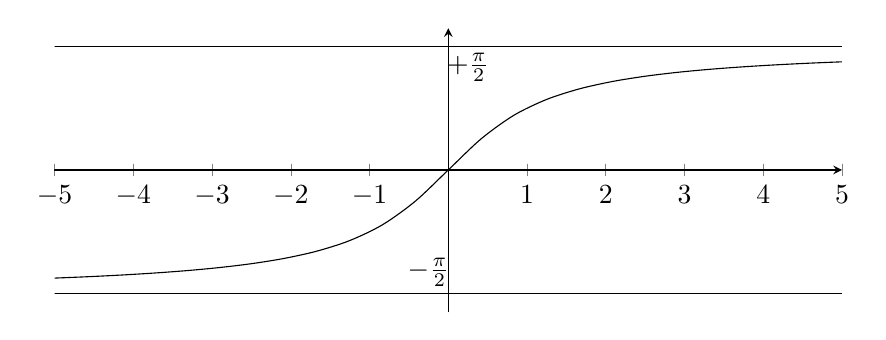
\begin{tikzpicture}[line cap=round,line join=round,>=triangle 45,x=1.0cm,y=1.0cm]
\begin{axis}[
x=1.0cm,y=1.0cm,
axis lines=middle,
ymajorgrids=false,
xmajorgrids=false,
xmin=-5.0,
xmax=5.0,
ymin=-1.8,
ymax=1.8,
xtick={-5.0,-4.0,...,5.0},
yticklabels=\empty,
ytick=\empty]
%ytick={-1.5707963267948966,0.0,...,1.5707963267948966},]
\clip(-5.,-1.7) rectangle (5.,1.7);

\draw[domain=-5.00:5.00] plot[smooth]({\x},{rad(atan(\x))}); 
\draw(-5.0,1.57)--(5.0,1.57);
\draw(-5.0,-1.57)--(5.0,-1.57);
\draw (0.25,1.3)node {$+\frac{\pi}{2}$};
\draw (-0.25,-1.3)node {$-\frac{\pi}{2}$};
\end{axis}
\end{tikzpicture}
\end{document}